\tikzsetnextfilename{figures/feinicial/feinicial}
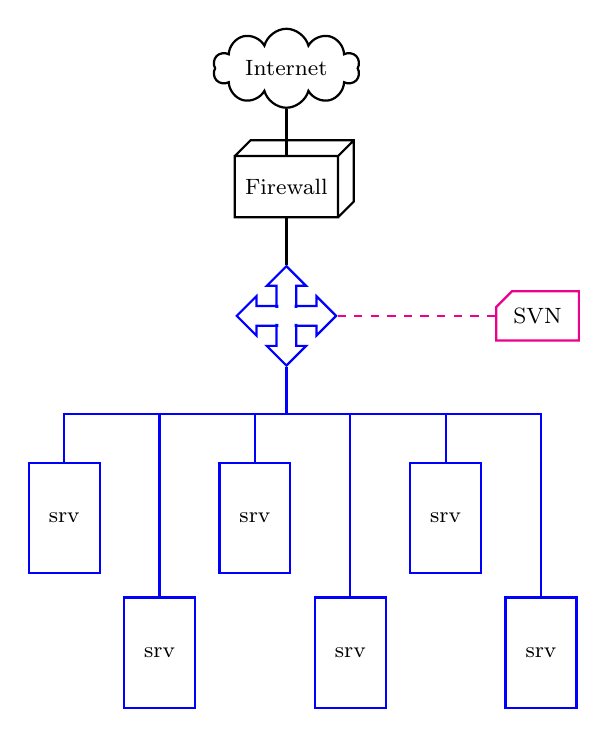
\begin{tikzpicture}[
    font=\footnotesize,
    thick
  ]
\usetikzlibrary{positioning,fit,calc,shapes}
\def\nw{1cm}

\makeatletter
\pgfkeys{/pgf/.cd,
  parallelepiped offset x/.initial=2mm,
  parallelepiped offset y/.initial=2mm
}
\pgfdeclareshape{parallelepiped}
{
  \inheritsavedanchors[from=rectangle] % this is nearly a rectangle
  \inheritanchorborder[from=rectangle]
  \inheritanchor[from=rectangle]{north}
  \inheritanchor[from=rectangle]{north west}
  \inheritanchor[from=rectangle]{north east}
  \inheritanchor[from=rectangle]{center}
  \inheritanchor[from=rectangle]{west}
  \inheritanchor[from=rectangle]{east}
  \inheritanchor[from=rectangle]{mid}
  \inheritanchor[from=rectangle]{mid west}
  \inheritanchor[from=rectangle]{mid east}
  \inheritanchor[from=rectangle]{base}
  \inheritanchor[from=rectangle]{base west}
  \inheritanchor[from=rectangle]{base east}
  \inheritanchor[from=rectangle]{south}
  \inheritanchor[from=rectangle]{south west}
  \inheritanchor[from=rectangle]{south east}
  \backgroundpath{
    % store lower right in xa/ya and upper right in xb/yb
    \southwest \pgf@xa=\pgf@x \pgf@ya=\pgf@y
    \northeast \pgf@xb=\pgf@x \pgf@yb=\pgf@y
    \pgfmathsetlength\pgfutil@tempdima{\pgfkeysvalueof{/pgf/parallelepiped offset x}}
    \pgfmathsetlength\pgfutil@tempdimb{\pgfkeysvalueof{/pgf/parallelepiped offset y}}
    \def\ppd@offset{\pgfpoint{\pgfutil@tempdima}{\pgfutil@tempdimb}}
    \pgfpathmoveto{\pgfqpoint{\pgf@xa}{\pgf@ya}}
    \pgfpathlineto{\pgfqpoint{\pgf@xb}{\pgf@ya}}
    \pgfpathlineto{\pgfqpoint{\pgf@xb}{\pgf@yb}}
    \pgfpathlineto{\pgfqpoint{\pgf@xa}{\pgf@yb}}
    \pgfpathclose
    \pgfpathmoveto{\pgfqpoint{\pgf@xb}{\pgf@ya}}
    \pgfpathlineto{\pgfpointadd{\pgfpoint{\pgf@xb}{\pgf@ya}}{\ppd@offset}}
    \pgfpathlineto{\pgfpointadd{\pgfpoint{\pgf@xb}{\pgf@yb}}{\ppd@offset}}
    \pgfpathlineto{\pgfpointadd{\pgfpoint{\pgf@xa}{\pgf@yb}}{\ppd@offset}}
    \pgfpathlineto{\pgfqpoint{\pgf@xa}{\pgf@yb}}
    \pgfpathmoveto{\pgfqpoint{\pgf@xb}{\pgf@yb}}
    \pgfpathlineto{\pgfpointadd{\pgfpoint{\pgf@xb}{\pgf@yb}}{\ppd@offset}}
  }
}
\makeatother


\node[cloud,cloud ignores aspect,draw,,minimum width=1.5*\nw,minimum height=\nw] (internet) {Internet};
\node[parallelepiped,draw,minimum width=\nw,minimum height=.75*\nw,node distance=.6*\nw,below = of internet] (firewall) {Firewall};
\node[arrow box,draw=blue,arrow box shaft width=.25*\nw,node distance=.6*\nw,below = of firewall] (redir) {};
\node[chamfered rectangle,chamfered rectangle corners=north west,draw=magenta,node distance=2*\nw,minimum width=.6*\nw,minimum height=.6*\nw,right = of redir] (svn) {SVN};
\coordinate (aux) at ($ (redir.south) - (0,.6*\nw) $);

% \tikzstyle{srv}=[cylinder,shape border rotate=90, shape aspect=0.4,minimum height=1.2*\nw,minimum width=0.8*\nw,node distance=.5*\nw]
\tikzstyle{srv}=[minimum height=1.4*\nw,minimum width=0.9*\nw,node distance=0.4*\nw]
\tikzstyle{blue}=[draw=blue]
\node[blue,srv,node distance=.6*\nw, below = of aux,xshift=-.4*\nw ] (srv1) {srv};
\node[blue,srv, below left = of srv1 ] (srv2) {srv};
\node[blue,srv, below right = of srv1 ] (srv3) {srv};
\node[blue,srv, above left = of srv2 ] (srv4) {srv};
\node[blue,srv, above right = of srv3 ] (srv5) {srv};
\node[blue,srv, below right = of srv5 ] (srv6) {srv};

\draw[-,blue] (srv1.north)  |- (aux) -- (redir.south);
\draw[-,blue] (srv2.north) |- (aux) -- (redir.south);
\draw[-,blue] (srv3.north) |- (aux) -- (redir.south);
\draw[-,blue] (srv4.north) |- (aux) -- (redir.south);
\draw[-,blue] (srv5.north) |- (aux) -- (redir.south);
\draw[-,blue] (srv6.north) |- (aux) -- (redir.south);

\draw[-,dashed,draw=magenta] (svn.west)  -- (redir.east);
\draw[-] (redir.north)  -- (firewall.south);
\draw[-] (firewall.north)  -- (internet.south);

%% \tikzstyle{agent}=[circle,draw,minimum height=.3*\nw,minimum width=.3*\nw,inner sep=0mm];
%% \node[agent] at ($ (srv1.south east) + (-.25*\nw,.25*\nw) $) (c1) {C};
%% \node[agent] at ($ (srv2.south east) + (-.25*\nw,.25*\nw) $) (c2) {C};
%% \node[agent] at ($ (srv3.south east) + (-.25*\nw,.25*\nw) $) (c3) {C};
%% \node[agent] at ($ (srv4.south east) + (-.25*\nw,.25*\nw) $) (c4) {C};
%% \node[agent] at ($ (srv5.south east) + (-.25*\nw,.25*\nw) $) (c5) {C};
%% \node[agent] at ($ (srv6.south east) + (-.25*\nw,.25*\nw) $) (c6) {C};

%% \tikzstyle{consul}=[circle,draw,minimum height=.6*\nw,minimum width=.6*\nw,inner sep=0mm];
%% \node[consul, node distance=1*\nw, left=of srv4]  (consul1) {C};
%% \node[consul, above=of consul1]  (consul2) {C};
%% \node[consul, above=of consul2]  (consul3) {C};
%% \node[consul, above=of consul3]  (consul4) {C};
%% \node[consul, above=of consul4]  (consul5) {C};

%% \coordinate (aux1) at ($ (srv4.south) - (0,2.2*\nw) $);
%% \coordinate (aux2) at ($ (consul2.east) + (0.2*\nw,0) $);
%% \coordinate (aux3) at ($ (consul3.west) - (0.2*\nw,0) $);

%% \draw[-,dashed] (c4.south)  |- (aux1) -| (aux2) -- (consul2.east);
%% \draw[-,dashed] (c3.south)  |- (aux1) -| (consul1.south);
%% \draw[-,dashed] (c2.south)  |- (aux1) -| (aux3) -- (consul3.west);
%% \draw[-,dashed] (c1.south)  |- (aux1);
%% \draw[-,dashed] (c5.south)  |- (aux1);
%% \draw[-,dashed] (c6.south)  |- (aux1);
%% \draw[-,dashed] (consul1.north)  -- (consul2.south);
%% \draw[-,dashed] (consul2.north)  -- (consul3.south);
%% \draw[-,dashed] (consul3.north)  -- (consul4.south);
%% \draw[-,dashed] (consul4.north)  -- (consul5.south);

%% \coordinate (aux4) at ($ (redir.west) - (\nw,0) $);
%% \draw[-,dashed] (consul4.east)  -| (aux4) -- (redir.west);

\end{tikzpicture}
